\documentclass[12pt]{article}
\title{Inferring generation-interval distributions from contact tracing data: \\ \emph{in prep, PRSB}}
\author{Sang Woo Park, David Champredon and Jonathan Dushoff}

\usepackage{graphics}
\usepackage{adjustbox}

\newcommand{\eref}[1]{(\ref{eq:#1})}
\newcommand{\fref}[1]{Fig.~\ref{fig:#1}}
\newcommand{\Fref}[1]{Fig.~\ref{fig:#1}}
\newcommand{\sref}[1]{Sec.~\ref{#1}}
\newcommand{\frange}[2]{Fig.~\ref{fig:#1}--\ref{fig:#2}}
\newcommand{\tref}[1]{Table~\ref{tab:#1}}
\newcommand{\tlab}[1]{\label{tab:#1}}

\usepackage{amsthm}
\usepackage{amsmath}
\usepackage{amssymb}
\usepackage{amsfonts}

\usepackage{hyperref}
\usepackage{natbib}
\usepackage{hyperref}
\bibliographystyle{chicago}
\date{\today}

\usepackage{xspace}
\newcommand*{\ie}{i.e.\@\xspace}

\usepackage{color}

\newcommand{\Rx}[1]{\ensuremath{{\mathcal R}_{#1}}} 
\newcommand{\Ro}{\Rx{0}}
\newcommand{\RR}{\ensuremath{{\mathcal R}}}
\newcommand{\Rhat}{\ensuremath{{\hat\RR}}}
\newcommand{\tsub}[2]{#1_{{\textrm{\tiny #2}}}}

\newcommand{\comment}[3]{\textcolor{#1}{\textbf{[#2: }\textsl{#3}\textbf{]}}}
\newcommand{\jd}[1]{\comment{cyan}{JD}{#1}}
\newcommand{\swp}[1]{\comment{magenta}{SWP}{#1}}
\newcommand{\dc}[1]{\comment{blue}{DC}{#1}}
\newcommand{\hotcomment}[1]{\comment{red}{HOT}{#1}}

\begin{document}
\maketitle

\section{Introduction}

An epidemic can be characterized by its speed (exponential growth rate, $r$) and its strength (reproductive number, \RR).
Reproductive number, defined as the average number of secondary cases arising from a primary case, is of particular interest as it provides information about the final size of an epidemic \citep{anderson1991infectious, diekmann1990definition}.
However, directly measuring the reproductive number often requires detailed knowledge of disease natural history and may not be feasible early in an epidemic [CITE].
Instead, the reproductive number can be \emph{indirectly} estimated from the exponential growth rate, which can often be estimated from incidence data \citep{mills2004transmissibility, nishiura2009transmission, ma2014estimating}.
These two quantities are linked by generation-interval distributions \citep{wallinga2007generation, park2019practical}.

Generation interval is defined as the time between when a person becomes infected and when that person infects another person.
Due to individual variation in infection time, the observed generation-interval distribution can change depending on when and how it is measured \citep{svensson2007note, kenah2008generation, nishiura2010time, champredon2015intrinsic}.
There are important distinctions to be made when estimating generation intervals: \emph{intrinsic} generation intervals are measured by evaluating the infectiousness of infected people,
%% without regard to actual infection events,
while \emph{observed} generation intervals refer to the time between actual infection events.
Observed generation intervals in turn can be \emph{aggregated} across time, measured \emph{forward} in time by looking at a cohort of individuals infected at the same time and asking when they infected others, or measured \emph{backward in time} by look at a cohort and asking when their infectors were infected \citep{champredon2015intrinsic}.
% When aggregated generation intervals are observed until a given time in an ongoing epidemic (often via contact tracing), we refer to these as \emph{censored} (or right-censored) intervals.

Early in the epidemic when depletion of susceptibles is negligible, we expect the forward generation-interval distribution to be similar to the intrinsic generation-interval distribution.
As epidemic progresses, an infector is less likely to infect individuals later in time due to decrease in susceptibles and the distribution of forward generation intervals will be shorter than the intrinsic distribution.
Conversely, when an epidemic is growing exponentially, as often occurs near the beginning of an outbreak, the number of newly infected individuals will be large relative to the number infected earlier on. 
A susceptible individual is thus relatively more likely to be infected by a newly infected individual, and the distribution of backward generation intervals will be shorter than the intrinsic distribution.
When epidemic is subsiding, most infections are caused by the remaining infectors, rather than new infectors, and the backward generation interval will be long \citep{champredon2015intrinsic}.

In practice, generation intervals are measured by contact tracing throughout the course of an epidemic, usually aggregated to increase the amount of information available; we refer to these as \emph{censored} (or right-censored) intervals.
When calculations are based on early-outbreak data, the available (censored) observations can be thought of as a weighted average of backward generation-interval distributions; like them, the observed censored intervals will be shorter than intrinsic distributions.

Observed generation intervals also vary across space.
In a structured population (that is, any population that does not mix homogeneously), susceptibility will tend to decrease more quickly in the neighborhood of infected individuals than in the general population. 
This means that contacts made late in infection are more likely to be ``masked'' due to contacts already being infected.
Therefore, realized generation intervals will be shorter and observed generation intervals may underestimate the intrinsic generation-interval distribution even when population-level susceptibility is very high.
This perspective allows us to reinterpret the finding of \cite{trapman2016inferring} that, given an intrinsic generation interval and an observed growth rate $r$, the reproductive number $\RR$ on various network structures is always smaller on a network than would be predicted from homogeneous mixing.

In this study, we explore the temporal and spatial variation in the observed generation-interval distributions obtained from contact tracing.
We show that directly using the \emph{observed} generation-interval distributions will generally underestimate the reproductive number \RR, while directly using \emph{intrinsic} generation-interval distributions (i.e., estimated from infectiousness profiles) will tend to overestimate \RR.
We discuss statistical approaches to estimating the effective generation-interval distributions and reproductive number of an outbreak from observed generation-interval distributions.

\swp{I might rename the sections later but I think I like the current order.}
\section{Generation-interval distributions across time}

\subsection{Intrinsic generation-interval distribution}

\begin{figure}[t]
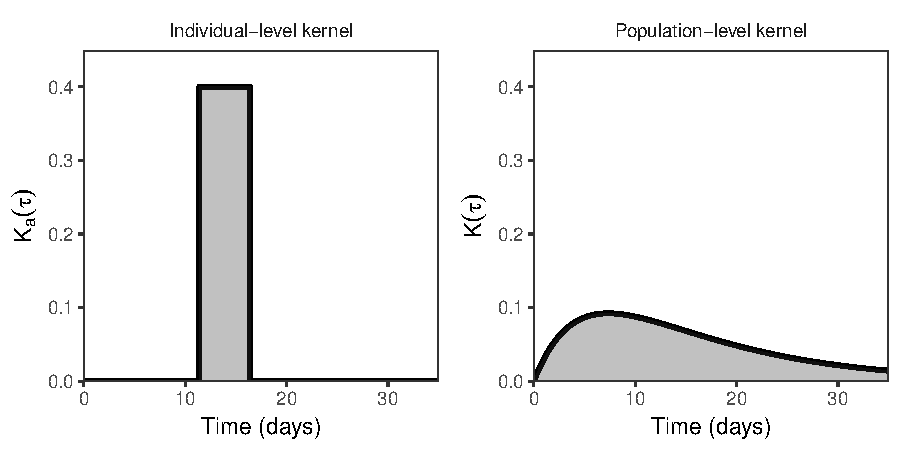
\includegraphics[width=\textwidth]{../fig/individual_and_population.pdf}
\caption{\textbf{Comparison of individual- and population-level kernels.}
(Left) an individual-level kernel of an infected individual with latent period of 11.4 days followed by infectious period of 5 days. 
(Right) a population-level kernal of infected individuals with exponentially distributed latent and infectious period of 11.4 and 5 days, respectively. 
Shaded areas under the curves are equal to individual- and population-level reproductive numbers, both of which are set to 2 in this example.
}
\label{fig:indpop}

\end{figure}

Generation-interval distributions are often viewed from a population-level pespective but we can distinguish population-level distributions from individual-level distributions (\fref{indpop}); 
making this distinction clear will be particularly useful when we discuss spatial components.
An individual-level intrinsic kernel $K_a(\tau)$ describes the rate at which secondary infections are expected to be caused by an infected individual $a$ \citep{svensson2007note, svensson2015influence}.
The population-level kernel is given by integrating over individual variations (e.g., variation in latent and infectious periods):
\begin{equation}
K(\tau) = \int K_a (\tau) dA.
\end{equation}
The population-level kernel describes the rate at which secondary infections are expected to be caused by an \emph{average} infected individual.
\jd{Do we need to worry about assumptions for the rest of this \P? Once we have an aspect space we need to assume that individual properties are independent of risk of infection. Also, since that's wrong on our networks, do we have to figure out why we're approximately saved? I guess because of scaling?}
\swp{What do you mean by individual properties?}

There are two components to infection kernels: intrinsic infectiousness of an infected individual (the basic reproductive number) and time distribution of new infections (generation-interval distribution).
The basic reproductive number -- average number of secondary cases caused by an \emph{average} primary case in a fully susceptible population -- is defined as: 
\begin{equation}
\RR_0 = \int K(t).
\end{equation}
The intrinsic generation-interval distribution is simply the population-level kernel normalized by the basic reproductive number:
\begin{equation}
g(\tau) = \frac{K(t)}{\RR_0}.
\end{equation}

Since the intrinsic generation-interval distribution describes time distribution of new infections, it can be used to model incidence over time:
\begin{equation}
i(\tau) = S(\tau) \int K(s) i(\tau-s) ds = \RR \int g(s) i(\tau-s) ds
\end{equation}
where $i(\tau)$ is incidence at time $\tau$ and $S(\tau)$ is the proportion of the population susceptible.
This model, also referred to as the renewal equation, represents wide range of epidemic models \citep{heesterbeek1996concept, diekmann2000mathematical, roberts2004modelling, aldis2005integral, wallinga2007generation, roberts2007model}.
Finally, assuming exponentially growing incidence ($i(t) = i(0) \exp(r t)$), we obtain the Euler-Lotka equation \citep{lotka1907relation}, which provides a direct link between speed and strength of an epidemic:
\begin{equation}
\frac{1}{\RR} = \int g(\tau) \exp(-r \tau) d\tau.
\end{equation}

\subsection{Right-censored generation-interval distribution}

\jd{Make sure we're not sounding too mathy.}
% For an emerging epidemic, it is reasonable to assume that contact tracing is performed from the beginning of an epidemic.
Assume that contact tracing is performed from the beginning of an epidemic to time $t$.
The number of infection occuring at time $s$ caused by infectors who were themselves infected at time $s-\tau$ is given by
\begin{equation}
i_{s-\tau}(s) = \RR i(s-\tau) g(\tau) S(s)
\end{equation}
Then, total number of secondary infections that are $\tau$ time steps apart and occur before time $t$:
\begin{equation}
\RR \int_\tau^t i(s-\tau) g(\tau) S(s) ds.
\end{equation}
Then, the censored generation-interval at time $t$ is given by
\begin{equation}
c_t(\tau)= \frac{\RR \int_\tau^t i(s-\tau) g(\tau) S(s) ds}{\RR \int_0^t \int_x^t i(s-x) g(x) S(s) ds dx}.
\end{equation}
The expression in the denominator is equivalent to cumulative incidence at time $t$; the intuition here is that we are normalizing acrosss all incidence before time $t$.
Then, we have
\begin{equation}
c_t(\tau) = \frac{\RR \int_\tau^t i(s-\tau) g(\tau) S(s) ds}{\int_0^t i(s) ds}.
\end{equation}
For convenience, we ignore normalizing constants and write
\begin{equation}\label{eq:obsg}
c_t(\tau) \propto g(\tau) \int_{0}^t i(s-\tau) S(s) ds.
\end{equation}

For a single epidemic, the observed mean generation interval through contact tracing will always be shorter than intrinsic mean generation interval (Figure~\ref{fig:censor}).
There are two reasons for this phenomenon.
First, any infection events that occur after the contact tracing period canonot be observed due to right censoring and short generation intervals are more likely to be observed.
In particular, when an epidemic is growing exponentially ($i(t) \propto \exp(rt)$), 
the censored generation-interval distribution is equivalent to the inverse exponentially weighted intrinsic generation-interval distribution:
\begin{equation}
\tsub{c}{exp}(\tau) \propto g(\tau) \exp(-r\tau).
\label{eq:exp}
\end{equation}
% As backward generation-interval distributions are always shorter than the intrinsic generation-interval distribution during the exponential growth period, their weighted average (i.e., the censored intervals) will also be shorter.
Second, decreasing number of susceptibles over the course of an epidemic makes long infections less likely to occur, and the realized intervals will always be shorter \citep{champredon2015intrinsic}.
As a result, even if contact tracing is performed through an entire epidemic, mean generation interval will be underestimated.

\begin{figure}
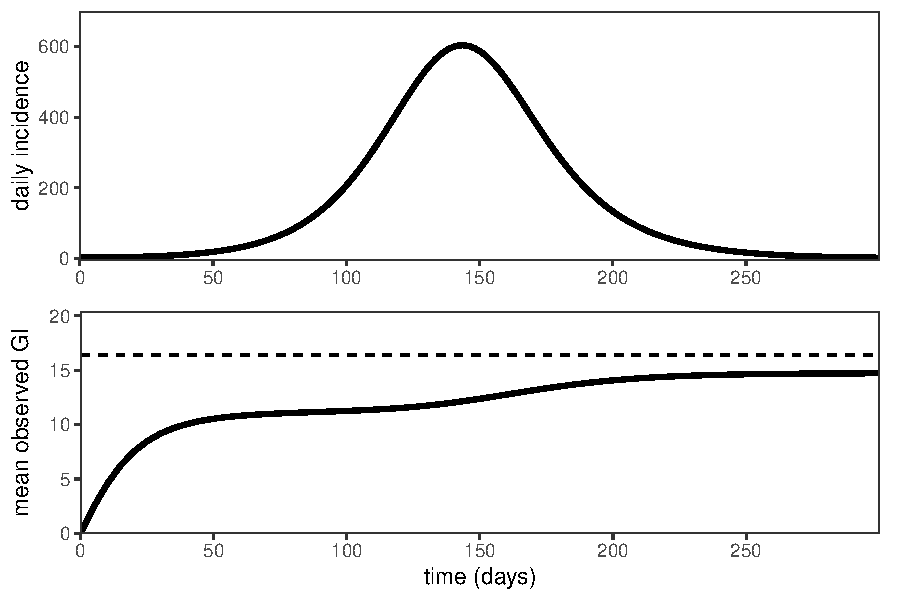
\includegraphics[width=\textwidth]{../fig/temporal_effect.pdf}
\caption{\textbf{Temporal variation in the mean observed generation interval.}
A deterministic Susceptible-Exposed-Infectious-Recovered (SEIR) model was simulated using Ebola-like parameters and the observed mean generation interval was calculated over the course of an epidemic (see methods).
\jd{Meaning, left-censored?}
}
\label{fig:censor}
\end{figure}

When a disease is at (or near) endemic equilibrium, the number of susceptibles remains (approximately) constant over time, and the observed generation-interval distribution should be similar to the intrinsic generation-interval distribution.
\swp{Probably don't need a figure for this}

\section{Generation-interval distributions across space}

\subsection{Egocentric kernel}

Within a limited contact structure, a susceptible individual can be contacted multiple times;
infectious contacts give rise to infection only when the susceptible individual is contacted for the first time.
In particular, we can look at it from an egocentric point of view -- i.e., from a perspective of a single infector.
We define the egocentric kernel, i.e., the rate at which secondary infections are realized by a single primary case $a$ in the absence of other infectors:
\begin{equation}
\hat{K}_a(\tau) = K_a(\tau) \exp \left(- \delta_a \int_0^\tau K_a(s) ds\right),
\end{equation}
where $K_a(\tau)$ is the individual-level intrinsic kernel and $e^{- \delta_a \int_0^\tau K_a(s) ds}$ is the probability that a susceptible acquaintance has not yet been contacted by individual $a$.
The dilution term, $\delta_a$, models how contacts are distributed among susceptible acquaintances.
For example, when infectious contacts are distributed equally in a homogeneous population, we have $\delta_a = 1/(N-1)$, where $N$ is the population size.

The population-level egocentric kernel is given by integrating over individual variations:
\begin{equation}
\hat{K}(\tau) = \int \hat{K}_a(\tau) dA,
\end{equation}
and the population-level egocentric generation-interval distribution is:
\begin{equation}
\hat{g}(\tau) = \frac{\hat{K}(\tau)}{\int \hat{K} \tau}.
\label{eq:conditional}
\end{equation}
The population-level egocentric generation-interval distribution describes the distribution of times at which secondary infections are realized by an average primary case.
For convenience, egocentric distribution refers to the population-level distribution, unless noted otherwise.

For example, consider a susceptible-exposed-infected-recovered (SEIR) model.
This model assumes that latent and infectious periods are exponentially distributed and can describe wide range of diseases.
It has been shown that the intrinsic generation-interval distribution that corresponds to this model is given by [CITE]:
\begin{equation}
g(\tau) = \frac{\sigma \gamma}{\sigma - \gamma} \left(e^{-\gamma t} - e^{-\sigma t}\right),
\end{equation}
where $1/\sigma$ and $1/\gamma$ are mean latent and infectious periods, respectively.
Assuming that per-pair contact rate is $\lambda$ for any pair, we obtain the following egocentric generation-interval distribution is given by:
\begin{equation}
\hat{g}(\tau) = \frac{\sigma (\gamma + \lambda)}{\sigma - (\gamma + \lambda)} \left(e^{-(\gamma + \lambda)t} - e^{-\sigma t}\right)
\end{equation}
In this scenario, per-pair contact rate effectively decreases mean infectious period: an infected individual can no longer infect anyone (hence no longer infectious) when all its susceptible acquaintances have ben infected.

The difference between egocentric and intrinsic generation-interval distribution can be demonstrated by simulating stochastic infection processes on a small tree network (i.e, a single infected individual is connected to multiple susceptible individuals who are not connected with each other) with artificially high per-pair contact rate.
Simulations confirm that in this case the distribution of contact times matches the intrinsic generation-interval distribution, while the distribution of realized generation times matches with the egocentric generation-interval distribution (\fref{local}) -- generation times are shorter on average because contacts with already-infected susceptibles do not lead to new infections.

\begin{figure}
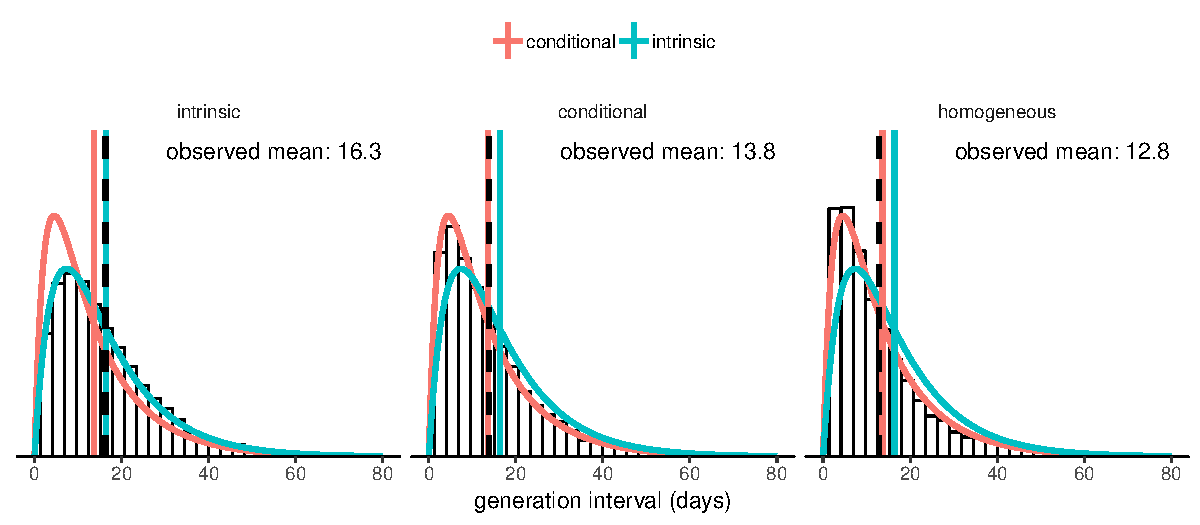
\includegraphics[width=\textwidth]{../fig/local_effect.pdf}
\caption{Fill this out.}
\label{fig:local}
\end{figure}

The egocentric generation interval \eref{conditional} only explains some of the reduction in generation times that occurs on most networks, however.
Generation intervals are also shortened by indirect connections: a susceptible individual can be infected through another route before the focal individual makes infectious contacts.
Simulations on a small homogeneous network confirm this additional effect (\fref{local}, right panel). 

In general, there are two factors that cause further reduction in the mean generation interval: (1) the local spatial effect (e.g., in a household) and (2) the overall depletion of susceptible individuals in the population;
the latter effect provides an equivalent explanation for the underestimation of the mean generation interval, sampled across an entire epidemic (\fref{censor}). 
Although the effect of the overall depletion of susceptible individuals is relatively well-understood \citep{champredon2015intrinsic}, estimating the effects of most networks on observed generation intervals is expected to be a hard problem. 
\jd{The global spatial effect is sort of the non-spatial effect: the overall response to decreasing susceptibles, like in Champredon.}
\swp{Tried to fix this}

\subsection{Linking growth rate and reproductive number}

The intrinsic generation-interval distribution provides a link between the speed (exponential growth rate, $r$) and the strength (reproductive number, $\RR$) of an epidemic via Euler-Lotka equation \citep{lotka1907relation} but assumes a homogeneously mixing population.
Instead, we can derive a relationship between $r$ and $\RR$ that accounts for the egocentric effect using the egocentric generation-interval distribution:
\begin{equation}
\frac{1}{\hat{\RR}} = \int \hat{g}(\tau) \exp(-r \tau) d\tau.
\end{equation}
This is equivalent to the relationship between $r$ and $\RR$ that \cite{trapman2016inferring} derived under a network structure. \swp{Need to confirm; Maybe prove it in appendix or something...how?}
As the egocentric distribution always has a shorter mean than the intrinsic distribution, \Rhat\ will always be smaller than $\RR$ estimated from the intrinsic distribution.
Similarly, \Rhat\ will always be greater than the \emph{true} reproductive number \RR\ as it does not account for other spatial effects that can decrease the mean generation interval.

\section{Inferring generation-interval distributions from a contact tracing data}

When generation intervals are sampled through contact tracing, there will be four effects present in the sample: (1) right-censoring effect, (2) egocentric effect, (3) local spatial effect and (4) mean susceptible depletion effect.
Right-censoring effect and egocentric effect are well-understood.
While the other two effects are difficult to measure, we can make qualitative predictions about their effects on the realized generation intervals and reproductive number. 
Both local spatial and susceptible depletion effects reduce number of infections that occur and shorten generation intervals but the time scale on which they matter differs:
local spatial effect will be important early in an epidemic whereas the susceptible depletion will be small until sufficient amount of susceptible individuals become infected.
As a result, we expect the initial spread of a disease and the realized reproductive number to be heavily dependent on local spatial and egocentric effects.

Since the right-censoring effect is a sampling artifact, it must be corrected for.
On the other hand, local and egocentric effects will be embedded within realized generation intervals and do not need to be corrected for as they reflect the unobserved characteristic of a realized epidemic.
We claim that accounting for the right-censoring effect is sufficient and any necessary spatial component will be accounted for implicitly.
Hereafter, we will refer to temporally corrected distribution as the effective generation-interval distribution to contrast from the intrinsic generation-interval distribution; only in a large homogeneously mixing population, the corrected generation-interval distribution will be equivalent to the intrinsic generation-interval distribution.
In this section, we investigate two statistical methods for correcting for temporal bias in a contact tracing data.
Detailed derivations of the two methods can be found in section ???.

We refer to the first method as the population-level method as it relies on the observed distribution aggregated across population.
As the observed generation-interval distribution is a weighted distribution of the effective distribution, the effective distribution can be recovered by taking the inverse of the weights, given by \eref{exp}.
Hence, the population-level method relies on the observed generation intervals and the exponential growth rate \citep{tomba2010some}:
\begin{equation}
g(\tau) \propto \tsub{c}{exp}(\tau) \exp(r\tau).
\end{equation}
While the population-level method is simple and intuitive, it does not use all available information from contact tracing data as it does not take into account who infected whom.

The individual-level method assumes that the initial exponential growth phase of an epidemic can be approximated by a Poisson process to derive a likelihood for the observations from each individual:
\begin{equation}
\mathcal{L}(\RR, \theta) = \prod_{j=1}^N \left(\RR^{n_j} \exp \left(- \RR \int_0^{\tsub{t}{censor} - t_j} g(s;\theta) ds \right) \prod_{i=1}^{n_j} g(\tau_{i, j}; \theta) \right),
\end{equation}
where $N$ is the total number of infected individuals, $n_j$ is the number of individuals infected by $j$, $\tsub{t}{censor}$ is the time period which censoring was performed until, $t_j$ is the time at which infector $j$ was infected, $\tau_{i,j}$ is the observed generation interval between infector $j$ and infectee $i$, and $\theta$ is the (vector) parameter of the generation-interval distribution $g$.
A similar method has beem proposed by \cite{forsberg2008likelihood} but it relies on discretized incidence reports rather than the observed generation intervals.

\swp{I might say something about independence transmission events in the results if I decide to compare forsberg2008 as well -- see forsberg 2008...}
\swp{I got stuck on forsberg 2008. I get weird estimates with wide confidence intervals but I feel like that's what their method is supposed to do (based on figure 3 in their paper). It doesn't use generation interval either so I think we can just ignore it?}
\jd{If it really is similar in some important way just stick with what you've already said. Otherwise, ignore it.}

First, we compare how the estimates from the two methods vary across time using a single stochastic simulation on a homogeneous network (Figure~\ref{fig:example}).
During the initial exponential growth period (approximately between 9 and 20 weeks), both population-level and individual-level methods yield similar estimates of mean generation interval and reproductive number.
However, we observe opposite trends after the growth period (approximately after 20 weeks).
As the population-level method takes a weighted average of the observed distribution, increase in the observed mean generation interval leads to increase in the nonparametric estimates of both mean generation interval and reproductive number.
On the other hand, as the individual-level method assumes a Poisson process with constant proportion of susceptibles, decrease in the number of susceptible is translated to underestimation of both mean generation interval and reproductive number.
we observe grdaual increase in the observed mean-generation interval as we aggregate more data, but using the raw observed generation interval distributions always underestimate both mean generation interval and reproductive number, as predicted from the deterministic simulation (Figure~\ref{fig:censor}).
Around the 14th week, reproductive number estimate based on the observed generation interval approximately matches the true reproductive number; this is due to initial overestimation of the initial growth rate and we generally expect reproductive to be underestimated. \swp{Maybe another figure in the supp}

\begin{figure}
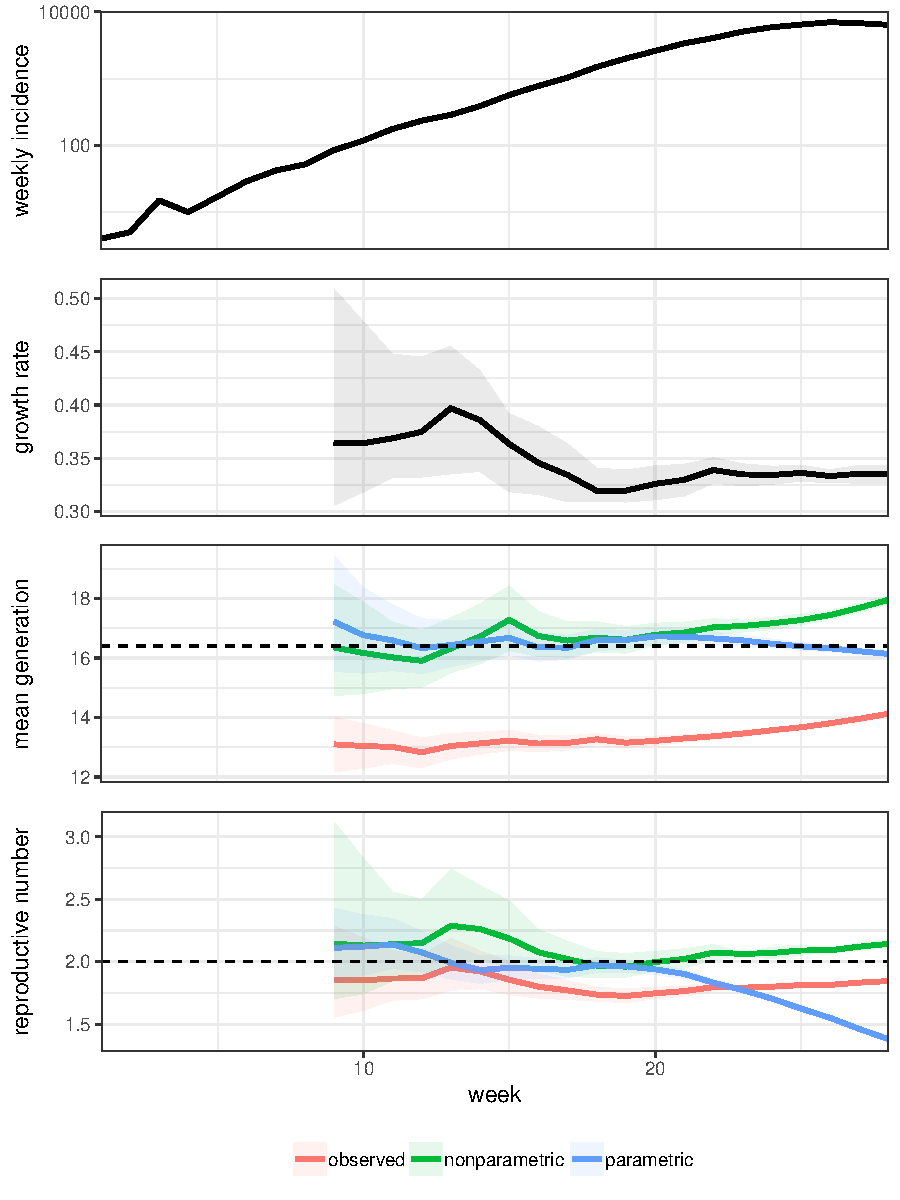
\includegraphics[width=\textwidth]{../fig/example.pdf}
\caption{Fill this out.}
\label{fig:example}
\end{figure}

We compare accuracy and reliability of the two methods during the initial growth period using 100 stochastic simulations on a homogeneous network (Figure~\ref{fig:test}).
We find that the individual-level method provides the most consistent (least variable) estimates.
The population method overestimates reproductive number initially but this is likely to be driven by the initial overestimation of the growth rate as discussed above (Figure~\ref{fig:example}).

\begin{figure}
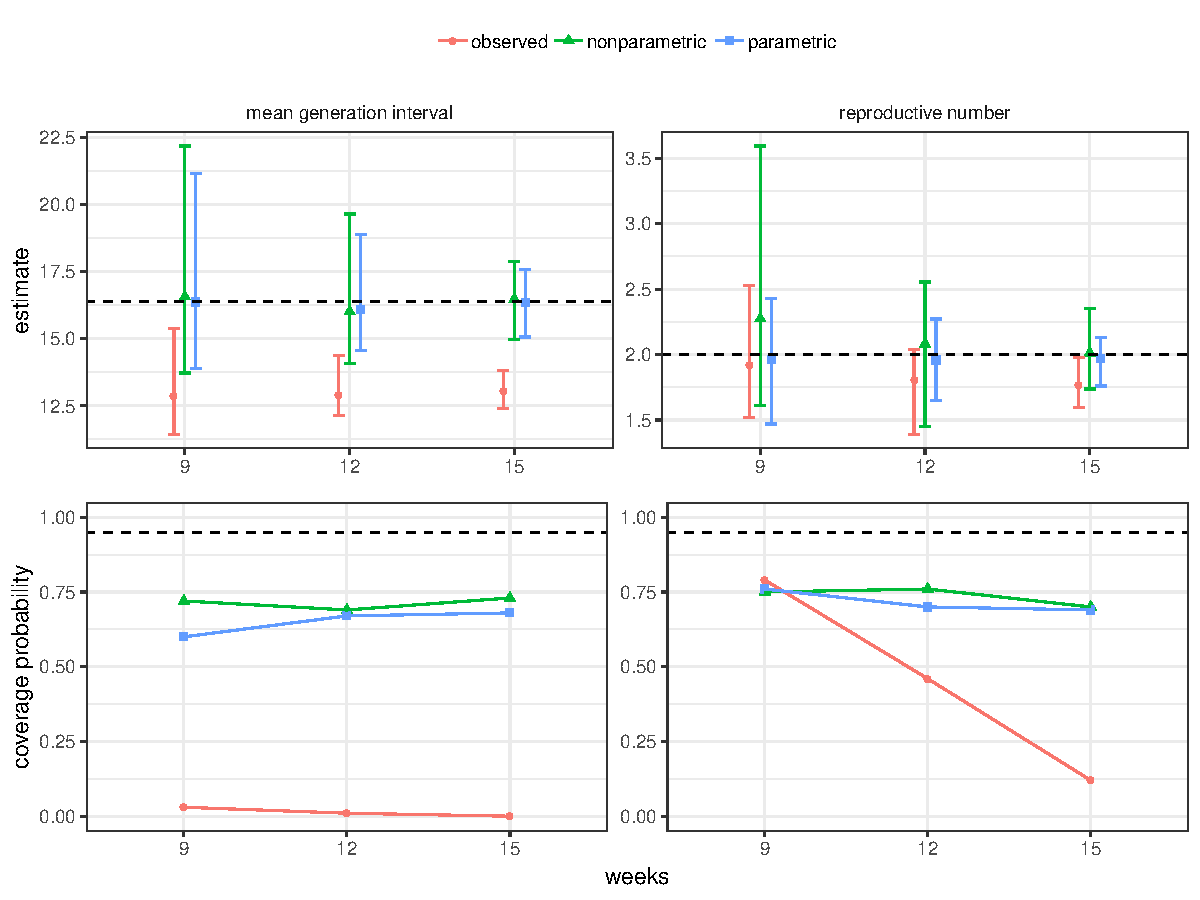
\includegraphics[width=\textwidth]{../fig/compare_methods.pdf}
\caption{Fill this out.}
\label{fig:test}
\end{figure}

We also compare coverage probabilities of these methods. 
Coverage probabilities are defined as the proportion of confidence intervals that contain the true value in a repeated simulations; for example, a 95\% confidence interval should attain 95\% coverage probability by its definition.
Surprisingly, both methods only attain approximately 70\% coverage.
Even though the gamma distribution looks indistinguishable from the shape of the intrinsic generation-interval distribution, making a wrong distributional assumption leads to narrow confidence intervals.
To confirm that the undercoverage is caused by distribuional assumption, we simulated an epidemic using gamma intrinsic generation-interval and found that fitting the true shape yields nominal coverage (see Appendix).
These results are particularly alarming because shape of the generation-interval distribution have often been assumed in outbreak analyses and it is impossible to know the true shape of the distribution [CITE].

\begin{figure}
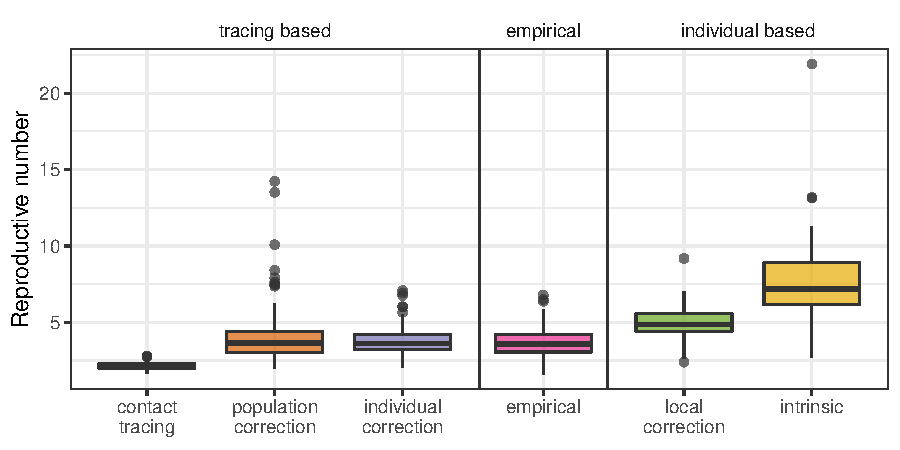
\includegraphics[width=\textwidth]{../fig/cmp_reproductive.pdf}
\caption{Fill this out.}
\label{fig:cmp}
\end{figure}

%% TODO: put SEIR in main text and show SE2IR in appendix for consistency
Finally, we simulate 100 epidemics with Ebola-liked parameters on an empirical network [CITE] and compare the estimates of reproductive number based on different methods with empirical reproductive numbers, which we define as the average number of secondary cases generated by the first 100 infected individuals (\fref{cmp}).
As we predicted earlier, calculating reproductive number based on the intrinsic generation-interval distribution overestimates the empirical reproductive number;
estimates based on the egocentric generation-interval distribution (\eref{conditional}) are closer to empirical reproductive numbers but still suffer from overestimation as they do not account for indirect spatial effects.
Direct estimates based on contact tracing data severely underestimates the empirical estimates.
Both population and individual corrections provide similar estimates to empirical reproductive numbers.
For smaller values of \RR, we expect the differences to become smaller. 

\clearpage

\section{Discussion}

\section{Methods}

The first method is a non-parametric method.
Recall that the observed generation-interval distribution is a weighted intrinsic generation-interval distribution (equation~\ref{eq:obsg}). 
Then, the intrinsic generation-interval distribution can be obtained by taking the inverse weight:
\begin{equation}
g(\tau) \propto c_t(\tau) \frac{1}{\int_{0}^t i(s-\tau) S(s) ds}
\end{equation}
However, this method requires a knowledge of susceptible dynamics and may difficult to use in practice.
Instead, during the exponential period, the generation-interval distribution is
\begin{equation}
g(\tau) \propto \tsub{c}{exp}(\tau) \exp(r\tau)
\end{equation}
and the reproductive number is
\begin{equation}
\RR = \int \tsub{c}{exp}(\tau) \exp(r\tau) d\tau.
\end{equation}
Note that applying the Lotka-Euler equation directly to the observed generation intervals will always underestimate the reproductive number:
\begin{equation}
\int_0^\infty \tsub{g}{exp}(\tau) \exp(r\tau) d\tau > \left(\int_0^\infty \tsub{g}{exp}(\tau). \exp(-r\tau) d\tau\right)^{-1}
\end{equation}

Finally, we obtain an estimator for mean generation interval and the reproductive number:
\begin{equation}
\begin{aligned}
\hat{G} &= \frac{\sum_{i} \exp(r c_i) c_i}{\sum_{i} \exp(r c_i)},\\
\hat{\RR} &= \sum_{i} \exp(r c_i),
\end{aligned}
\end{equation}
where $r$ is the exponential growth rate and $c_i$ is an individual generation interval sample.

\section{Appendix}

These are notes for now ... Need to move them elsewhere and change notation... but this is part of our figure for empirical network ...

$$
1 = \kappa \phi_L(\alpha) \frac{\lambda^{(net)}}{\alpha + \lambda^{(net)}} (1 - \phi_I(\alpha+\lambda^{(net)}))
$$
where in our specific example,
$$
\phi_L(\alpha) = \frac{4 \delta^2}{(2 \delta + \alpha)^2}
$$
and so we have
$$
1 = \frac{4 \delta^2}{(2 \delta + \alpha)^2} \frac{\kappa \lambda^{(net)}}{\lambda^{(net)} + \alpha + \gamma},
$$
which suggests that
$$
\lambda^{(net)} = \frac{(2\delta + \alpha)^2 (\alpha + \gamma)}{(\kappa - 1) 4 \delta^2 - 4 \delta \alpha - \alpha^2}
$$
We can substitute into the following equation to obtain the $r$ and $\RR$ relationship:
$$
\RR = \kappa \frac{\lambda^{(net)}}{\lambda^{(net)} + \gamma}
$$

\bibliography{network}
\end{document}
